\part{LED简介}

% https://en.wikipedia.org/wiki/Light-emitting_diode

\begin{slide}
  ~\vspace{-3em}\\
  \begin{multicols}{2}
    \parbox{\textwidth}{
      \parbox{\columnwidth}{
        ~\\~\\
        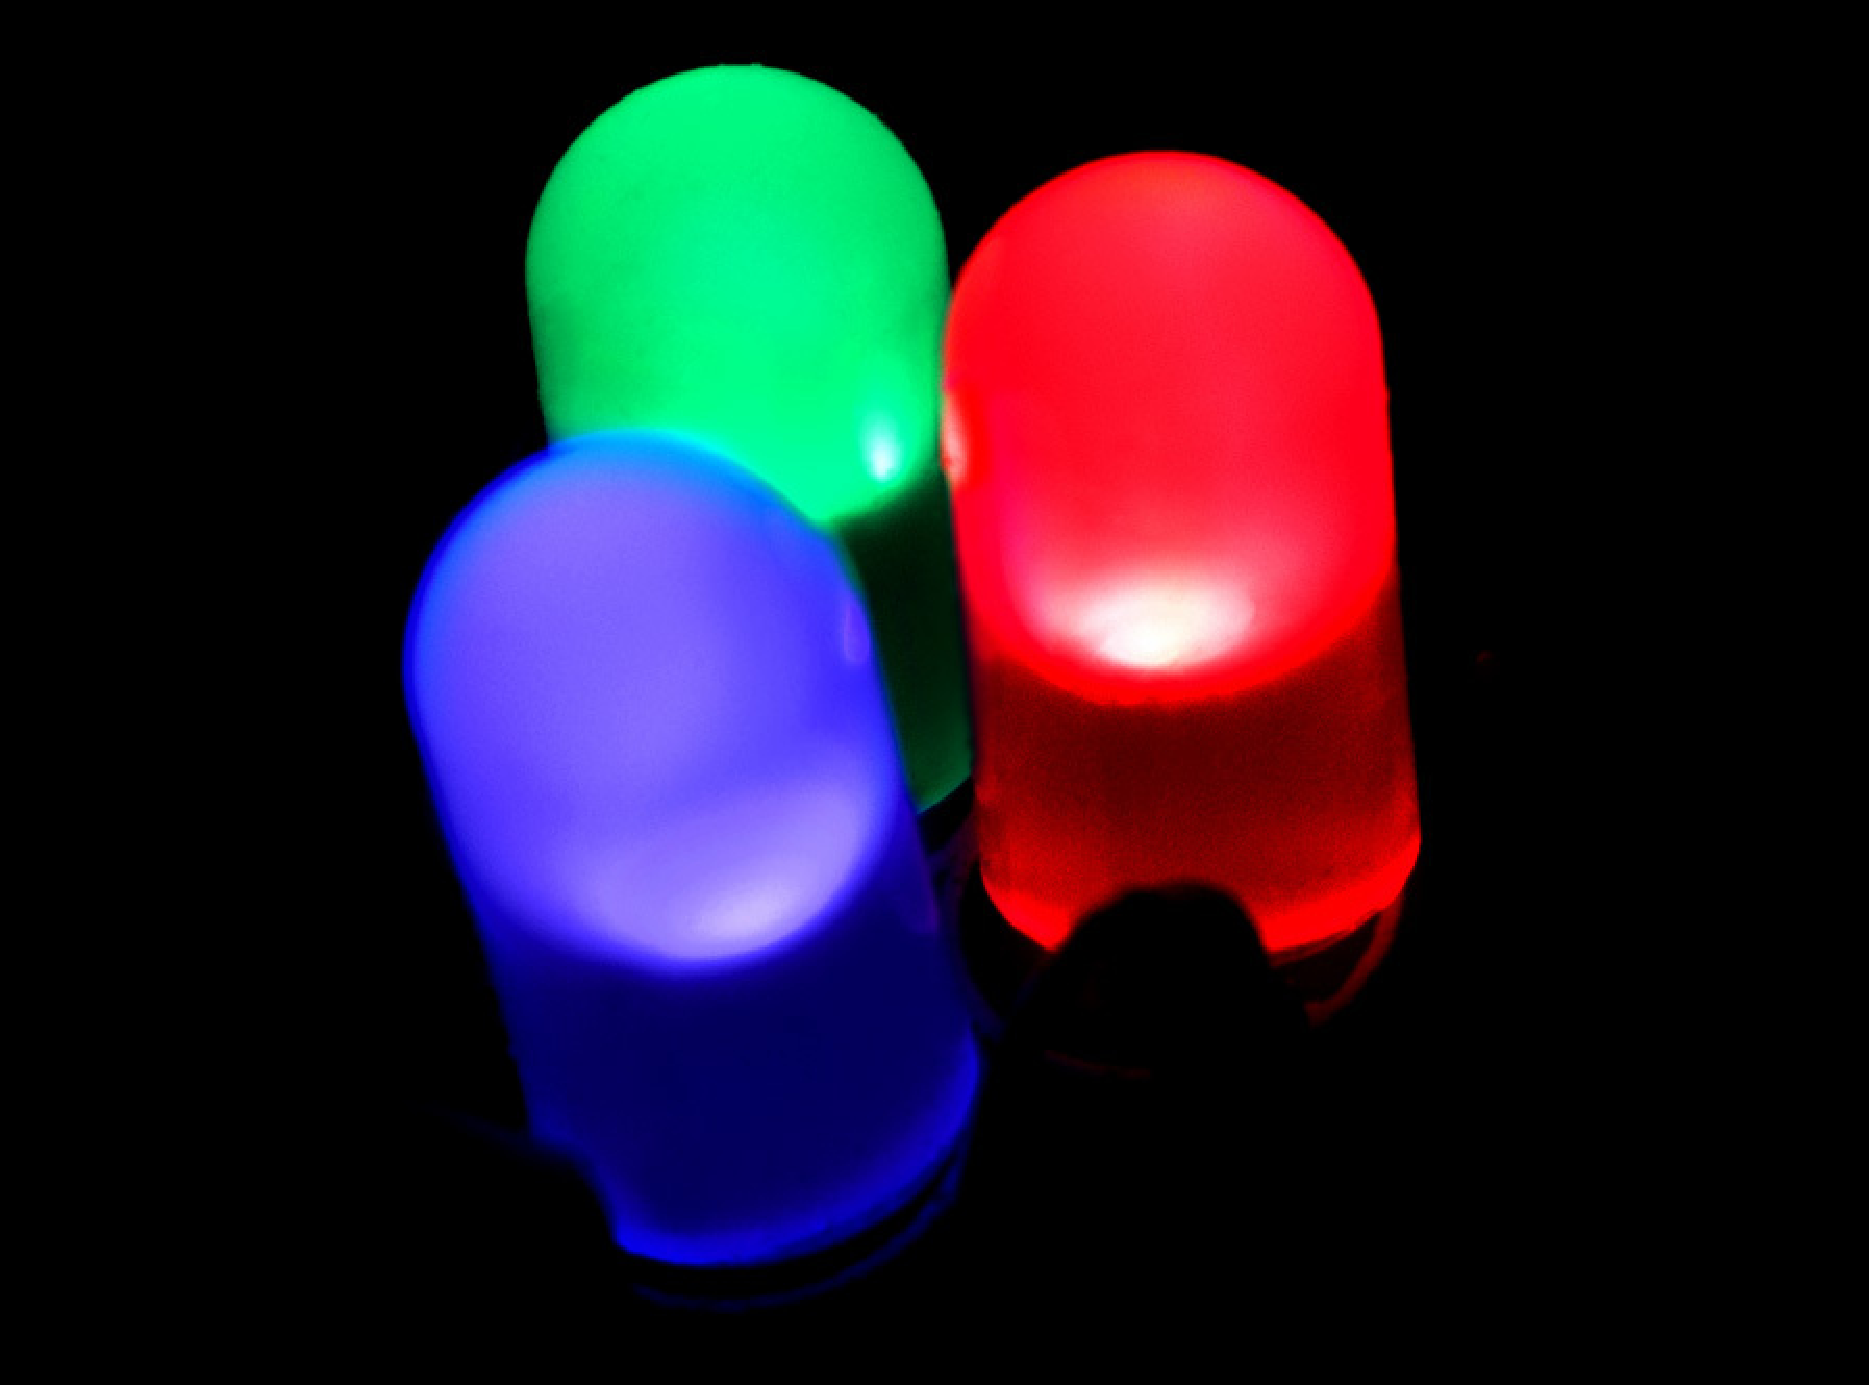
\includegraphics[width=\columnwidth]{sep3_images/RBG-LED.pdf}
      }
      \parbox{\columnwidth}{
        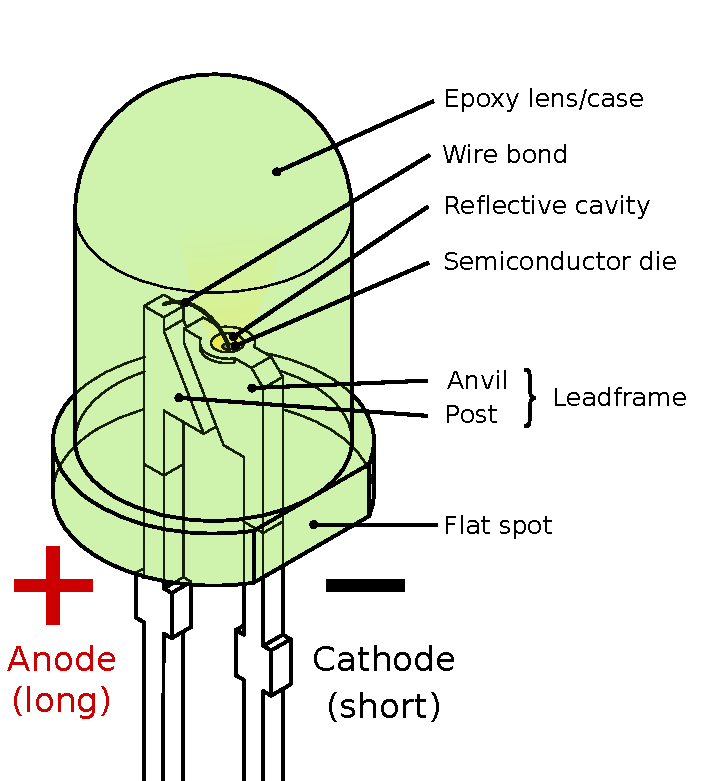
\includegraphics[width=\columnwidth]{sep3_images/LED,_5mm,_green_(en).pdf}
      }
    }
  \end{multicols}
  \url{https://en.wikipedia.org/wiki/Light-emitting_diode} \\
  Anvil(?), Post(?), Leadframe(引线框架), die(芯片), Reflective cavity(反射腔), Wire bond(焊线), Epoxy case(环氧树脂外壳)
\end{slide}

\section{何为LED}

\begin{slide}
  A light-emitting diode (LED) is a semiconductor light source that emits light when current flows through it. Electrons in the semiconductor recombine with electron holes, releasing energy in the form of photons. The color of the light (corresponding to the energy of the photons) is determined by the energy required for electrons to cross the band gap of the semiconductor. White light is obtained by using multiple semiconductors or a layer of light-emitting phosphor on the semiconductor device.
  \\~\\
  发光二极管（LED）是一种\textbf{通电时发光的半导体光源}。半导体中的电子和空穴重新结合时以光子的形式释放出能量。光的颜色（与光子的能量对应）由电子穿过半导体的能带空隙所需的能量决定。白光由多种半导体同时发光或由一层发光磷光体在半导体设备上获得。
  % TODO 什么是磷光体
\end{slide}

\section{LED发展历史}

\begin{slide}
  Appearing as practical electronic components in 1962, the earliest LEDs emitted low-intensity infrared (IR) light. Infrared LEDs are used in remote-control circuits, such as those used with a wide variety of consumer electronics. The first visible-light LEDs were of low intensity and limited to red. Early LEDs were often used as indicator lamps, replacing small incandescent bulbs, and in seven-segment displays.
  \\~\\
  最早的发光二极管于1962年作为实际使用的电子元件出现，可发出\textbf{低亮度的红外光}。红外LED被用于遥控电路中，例如制造各种各样的电子消费品。最早的可见光LED亮度低，且局限于红光。早期LED常用作台灯指示灯，替代原先的小白炽灯，以及制造七段数码显示管。
\end{slide}

\begin{slide}
  Recent developments have produced LEDs available in visible, ultraviolet (UV), and infrared wavelengths, with high, low, or intermediate light output, for instance white LEDs suitable for room and outdoor area lighting. LEDs have also given rise to new types of displays and sensors, while their high switching rates are useful in advanced communications technology with applications as diverse as aviation lighting, fairy lights, automotive headlamps, advertising, general lighting, traffic signals, camera flashes, lighted wallpaper, horticultural grow lights, and medical devices.
  \\~\\
  近期发展出多种LED，包括\textbf{可见光、紫外光、红外光波段，覆盖低中高各亮度}，对室内和室外空间均有适配。随LED还发展出多种显示和传感技术，其高转换速率在先进通信技术中大有用途，包括航空照明、小彩灯、汽车头灯、广告、一般照明、交通信号灯、相机闪光灯、发光墙纸、园艺灯和医学设备等。
\end{slide}

\section{LED的优劣}

\begin{slide}
  LEDs have many advantages over incandescent light sources, including lower power consumption, longer lifetime, improved physical robustness, smaller size, and faster switching. In exchange for these generally favorable attributes, disadvantages of LEDs include electrical limitations to low voltage and generally to DC (not AC) power, inability to provide steady illumination from a pulsing DC or an AC electrical supply source, and lesser maximum operating temperature and storage temperature.
  \\~\\
  相比白炽灯光源，LED有众多优势，比如更低功率损耗、更长寿命、更好的物理鲁棒性、更小的体积和更快的切换本领。作为补偿，LED的缺点包括低电压局限和直流电供电局限，在脉动直流电或交流电源下无法稳定发光，且最高工作和储存温度较低等。
\end{slide}

\begin{slide}
  In contrast to LEDs, incandescent lamps can be made to intrinsically run at virtually any supply voltage, can utilize either AC or DC current interchangeably, and will provide steady illumination when powered by AC or pulsing DC even at a frequency as low as 50 Hz. LEDs usually need electronic support components to function, while an incandescent bulb can and usually does operate directly from an unregulated DC or AC power source.
  \\~\\
  与LED相比，白炽灯固有地在几乎任意的供电电压下都可以工作，可以交替使用交流或直流电，在频率低至50赫兹的交流电或脉动直流电下仍能提供稳定照明。LED发光通常\textbf{需要其他电子元件的支持}，但白炽灯可以且通常直接接到非受控直流电源或交流电源上工作。
\end{slide}
